\section{Directly Generating Input Model}
\label{app:sec:directly_generating_input}
In this section, we present our model generating pseudo contexts directly in the input space.
We will present two kinds of model structure, i) directly generating pseudo context pair $(x,y)$ simultaneously by ISAB, ii) generating pseudo context data $x$ and $y$, sequentially. 
\subsection{Construction}
\paragraph{Generating pseudo context pair simultaneously.}
The generator of our first model which simultaneously generating pseudo context pair $(x',y')$, takes real context dataset $Z_c$ as input and outputs pseudo context dataset $Z'$. 
Here the generator is the one layer ISAB module.
Then we concatenate $Z_c$ and $Z'$ in order to treat this concatenated set as context dataset.
Then the encoder takes this concatenated context set as input.
And the others are the same with \gls{cnp} or \gls{canp}.
\paragraph{Sequentially generating pseudo context data \texorpdfstring{$x$}{x} and \texorpdfstring{$y$}{y}}
In this model, the generator takes real context dataset $Z_c$ as input and outputs only $x'$s of $Z'$. 
Here the generator is the one layer ISAB module with additional one linear layer.
Then we consider these $x'$s as our target dataset and find the mean and variance of $y'$ for each $x'$ by forwarding the model with context dataset $Z_c$ and target $x'$.
We sample $y'$ from the Gaussian distribution with mean and variance from the prior step.
We again concatenate $Z_c$ with $Z'$ and use them as context dataset.

\paragraph{Training}
Having directly generated a pseudo context set, we construct our empirical density as
\[
g_N(z) = \frac{1}{N}\bigg(\sum_{i\in c}\delta_{z_i}(z) + \sum_{i=1}^{N-|c|} \delta_{z'_i}(z)\bigg).
\]
Given $g_N$, we find the function parameter $\theta$ as
\[
\theta(g_N) := \argmin_\theta \int \ell(z, \theta) g_N(dz),
\]
where we simply choose $l(z,\theta):=-\log \calN (y|\mu_\theta(x),\sigma_\theta^2(x)I_{d_{out}})$.
In order to train the directly generating input model, which well approximate $\theta(g_N)$, we should construct different objective function from \cref{eq:mpnp_term_whole} because we can compute the exact $\int \ell(z, \theta) g_N(dz)$, unlike the feature generating model.
First, we approximate the marginal likelihood which is,
\[
\label{eq:direct1}
\log p(Y|X, Z_c) \approx \log \Bigg[ \frac{1}{K} \sum_{k=1}^K \exp\bigg(-\sum_{i\in [n]}\ell(z_i, \tilde\theta(Z_c\cup Z'^{(k)}))\bigg)
\Bigg] := -\calL_\text{marg}(\tau,\phi),
\]
where $Z'^{(1)},\dots, Z'^{(K)}\iidsim p(Z'|Z_c;\phi_\text{pred})$.
\cref{eq:direct1} is the same training object with \cref{eq:mpnp_term1}.
As we mentioned in \cref{main:subsec:training}, if we are given sufficiently well approximated $\Tilde{\theta}(Z_c\cup Z^{'(K)})$ then this objective would be suffice. However only with \cref{eq:direct1}, we cannot train the encoder to properly amortize the parameter construction process \cref{eq:recovering_theta}. To overcome this issue, we use $\int \ell(z, \theta) g_N(dz)$ as our second training objective which is,
\[
\label{eq:direct2}
\frac{1}{K}\sum_{k=1}^K\int \ell(z,\theta)g_N^{(k)}(dz) = \frac{1}{K}\sum_{k=1}^K\sum_{z\in Z_c\cup Z^{'(k)}} \Big(-\ell \big(z, \tilde{\theta}(Z_c\cup Z^{'(k)}\big)\Big)
:= \calL_\text{amort}(\tau,\phi).
\]
Combining these two functions, our loss function for the direct \gls{mpnp} is then
\[
\bbE_{\tau}[\calL(\tau,\phi)] = \bbE_\tau[\calL_\text{marg}(\tau,\phi) + \calL_\text{amort}(\tau,\phi)].
\]

\subsection{Sample}
% \begin{figure}[t]
%     \centering
%     \includegraphics[width = 0.32\textwidth]{figure/sample plot 9 xy without pseudo.pdf}
% %     \includegraphics[width = 0.32\textwidth]{figure/sample plot 9 xy.pdf}
% %     \includegraphics[width = 0.32\textwidth]{figure/sample plot 9 residual.pdf}
% %     % \includegraphics[width = 0.32\textwidth]{figure/data plot 9.pdf}
% %     % \includegraphics[width = 0.32\textwidth]{figure/sample plot 9.pdf}
% %     % \includegraphics[width = 0.32\textwidth]{figure/posterior plot 9.pdf}
% %     \caption{Generated pseudo context data samples of MPANP in 1d regression task. (Left) Generated pseudo context samples from simultaneously generating model without the term $\calL_{\text{amort}}$ in the loss $\calL$. (Middle) Generated pseudo context samples from simultaneously generating model after adding the term $\calL_{\text{amort}}$ in the loss $\calL$. (Right) Generated pseudo context samples from sequentially generating model.} 
% %     \label{fig:direct}
% \end{figure}
\begin{table}[t]
\centering

\caption{Test results for 1D regression tasks on RBF. `Context' and `Target' respectively denote context and target log-likelihood values, and `Task' denotes the task log-likelihood. All values are averaged over four seeds.}
\label{table/app_gp_inf_direct}
\begin{tabular}{lrrr}
\toprule
& \multicolumn{3}{c}{RBF}  \\
\cmidrule(lr){2-4}
Model & Context & Target & Task  \\
\midrule
CNP & 1.096$\spm{0.023}$ &  0.515$\spm{0.018}$ &  0.796$\spm{0.020}$ \\
NP  & 1.022$\spm{0.005}$ &  0.498$\spm{0.003}$ &  0.748$\spm{0.004}$ \\
BNP & 1.112$\spm{0.003}$ &  0.588$\spm{0.004}$ &  0.841$\spm{0.003}$ \\
\textBF{MPNP (ours)} & 
\textBF{1.189}$\spm{0.005}$ & \textBF{0.675}$\spm{0.003}$ & \textBF{0.911}$\spm{0.003}$ \\
\textBF{MPNP DSI(ours)} & 
1.120$\spm{0.007}$ & 0.551$\spm{0.006}$ & 0.822$\spm{0.007}$ \\
\textBF{MPNP DSE(ours)} & 
1.121$\spm{0.007}$ & 0.555$\spm{0.006}$ & 0.824$\spm{0.007}$ \\
\midrule
CANP & 
 1.304$\spm{0.027}$ &  0.847$\spm{0.005}$ &  1.036$\spm{0.020}$  \\
ANP & 
 \textBF{1.380}$\spm{0.000}$ &  0.850$\spm{0.007}$ &  1.090$\spm{0.003}$  \\
BANP & 
 \textBF{1.380}$\spm{0.000}$ &  0.846$\spm{0.001}$ &  1.088$\spm{0.000}$  \\
\textBF{MPANP (ours)} & 
 1.379$\spm{0.000}$ &  \textBF{0.881}$\spm{0.003}$ &  \textBF{1.102}$\spm{0.001}$ \\
 \textBF{MPANP DSI(ours)} & 
 \textBF{1.380}$\spm{0.000}$ &  0.796$\spm{0.013}$ &  1.069$\spm{0.005}$ \\
  \textBF{MPANP DSE(ours)} & 
 1.380$\spm{0.000}$ &  0.783$\spm{0.014}$ &  1.064$\spm{0.005}$ \\
\bottomrule
\end{tabular}
\end{table}


\begin{figure}[t]
    \centering
    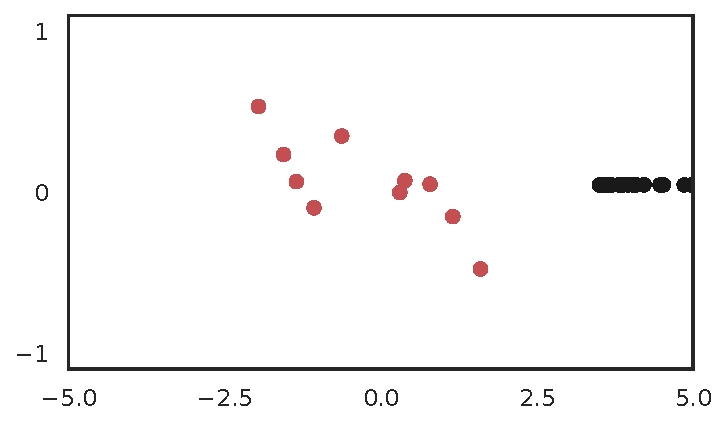
\includegraphics[width = 0.49\textwidth]{figure/direct2_pseudo.pdf}
    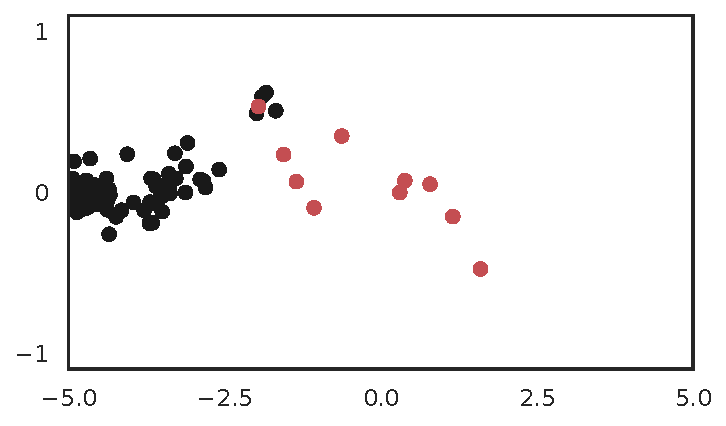
\includegraphics[width = 0.49\textwidth]{figure/direct8_pseudo.pdf}
    % \includegraphics[width = 0.32\textwidth]{figure/data plot 9.pdf}
    % \includegraphics[width = 0.32\textwidth]{figure/sample plot 9.pdf}
    % \includegraphics[width = 0.32\textwidth]{figure/posterior plot 9.pdf}
    \caption{It shows generated pseudo context dataset of direct \gls{mpanp} for 1D regression task with RBF kernel. The red dots are true context points sampled from \gls{gp} with RBF kernel, and the black dots are generated pseudo context points. (Left) Results from simultaneously generating pseudo context pair \gls{mpanp} model. (Right) Results from sequentially generating pseudo context data \gls{mpanp} model.}
    \label{fig:direct_sample}
\end{figure}
\begin{figure}[t]
    \centering
    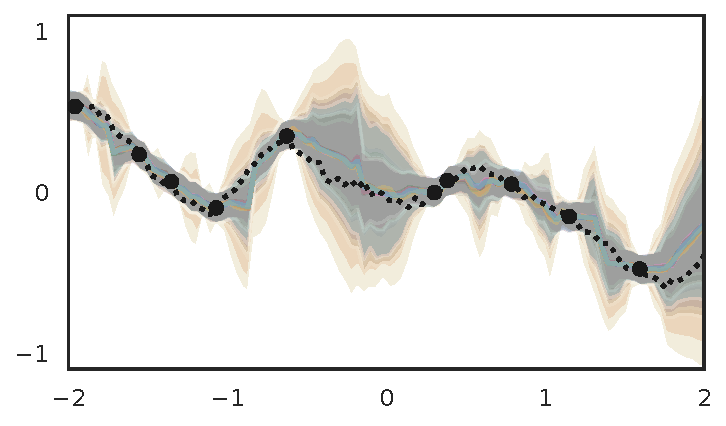
\includegraphics[width = 0.49\textwidth]{figure/direct2.pdf}
    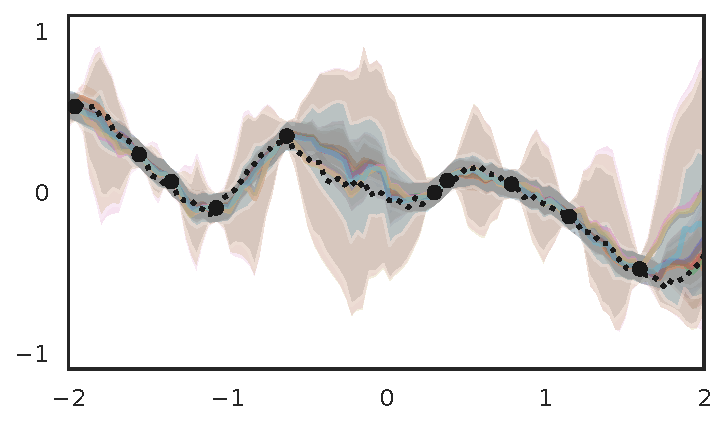
\includegraphics[width = 0.49\textwidth]{figure/direct8.pdf}
    % \includegraphics[width = 0.32\textwidth]{figure/data plot 9.pdf}
    % \includegraphics[width = 0.32\textwidth]{figure/sample plot 9.pdf}
    % \includegraphics[width = 0.32\textwidth]{figure/posterior plot 9.pdf}
    \caption{It shows posterior samples of direct \gls{mpanp} for 1D regression task with RBF kernel. The black dashed line is a function sampled from \gls{gp} with RBF kernel, and the black dots are context points. We visualized decoded mean and standard deviation with colored lines and areas. (Left) Results from simultaneously generating pseudo context pair \gls{mpanp} model. (Right) Results from sequentially generating pseudo context data \gls{mpanp} model.}
    \label{fig:direct_decode}
\end{figure}

In this section, we presents how the directly generating input model actually samples the pseudo context datasets. 

In \cref{fig:direct_sample}, we report generated pseudo context datasets and posterior samples from two different cases of directly generating input models for 1D regression task with RBF kernel. Here we can see that the generator samples pseudo context datasets far from the real context dataset. This phenomenon occurs because the generator learns to generate meaningless inputs ignored by the decoder.
In \cref{fig:direct_decode}, we report how two different directly generating \glspl{mpanp} predict posterior samples for 1D regression task with RBF kernel. 
Although directly generated pseudo context dataset are a bit far from context dataset, our model still well capture the functional uncertainty in this case.
We report the test results for 1D regression tasks on RBF for two directly generating models in \cref{table/app_gp_inf_direct}.
DSI and DSE indicate simultaneously generating models and sequentially generating models, respectively.
\cref{table/app_gp_inf_direct} shows that our directly generating models still outperform \gls{cnp} and \gls{canp} in the perspective of log-likelihood.

% In \cref{fig:direct}, we report generated pseudo context dataset from three different cases of directly generating input model.
% The first figure on the left of the \cref{fig:direct} shows the generated pseudo context samples from simultaneously generating model without the term $\calL_{\text{amort}}$ in the loss $\calL$.
% Here, we can see that the generator learns to generate meaningless inputs that are ignored by the decoder.
% The second figure on the middle of the \cref{fig:direct} shows the generated pseudo context samples from simultaneously generating model after adding the term $\calL_{\text{amort}}$ in the loss $\calL$.
% In this figure, we can see that although the model generates much more meaningful pseudo context dataset compare to the first one, still the generator fails to make sufficiently reasonable pseudo context dataset.
% The third figure on the right of the \cref{fig:direct} shows the generated pseudo context samples from sequentially generating model.
% In this figure, we can see that the model generates sufficiently meaningful pseudo context dataset compare to the others but it generates overconfidently for the unseen data points.
% Thus it fails to capture the functional uncertainty of the model which occurs the lack of the performance.
% \subsection{Long Training}